% =====================================================================
% PHASE 2 TAGGED DRAFT — CP219 AI Text Detection Report
% =====================================================================
% TAGGING KEY:
%   [GREEN]  — definitely include (core results, final numbers, defining decisions)
%   [YELLOW] — include if space allows (secondary detail, supporting experiments)
%   [RED]    — cut first under space pressure (background, repetition, minor/rejected)
%
% TBDs and conflicts are marked:  **TBD**, **FLAG**, **INCONSISTENCY**
%
% PLOT DIRECTIVE APPLIED:
%   INCLUDE:  Plots 11, 9, 8, 7, 6
%   INCLUDE (YELLOW): Plot 2 (user unsure due to space)
%   EXCLUDE:  Plots 5, 12
%   Old plots from previous report draft (baseline_progression.png, cv_vs_lb.png) REMOVED
% =====================================================================

\documentclass[11pt]{article}

% --- Page geometry (>=1cm margins per spec) ---
\usepackage[margin=1.2cm, top=1.2cm, bottom=1.2cm]{geometry}

% --- Packages ---
\usepackage{amsmath, amssymb}
\usepackage{graphicx}
\usepackage{booktabs}
\usepackage{multirow}
\usepackage{enumitem}
\usepackage[font=small, labelfont=bf]{caption}
\usepackage{xcolor}
\usepackage{hyperref}
\usepackage{subcaption}

% --- Compact spacing ---
\usepackage{titlesec}
\titlespacing*{\section}{0pt}{6pt}{3pt}
\titlespacing*{\subsection}{0pt}{4pt}{2pt}
\titleformat{\section}{\normalfont\bfseries\large}{\thesection.}{0.5em}{}
\titleformat{\subsection}{\normalfont\bfseries\normalsize}{\thesubsection}{0.5em}{}
\setlength{\parskip}{2pt}
\setlength{\parindent}{0pt}
\setlength{\abovecaptionskip}{4pt}
\setlength{\belowcaptionskip}{2pt}
\setlist{nosep, leftmargin=1.2em}
\renewcommand{\arraystretch}{1.05}

\begin{document}

% =====================================================================
% FRONT MATTER [GREEN]
% =====================================================================
\begin{center}
    {\Large\bfseries Human vs.\ Machine Text Classification\\[2pt]on Obfuscated Token Sequences}\\[6pt]
    {\normalsize CP219 Machine Learning --- Project~1}\\[2pt]
    {\normalsize Author Name \quad | \quad IISc, Semester 1, 2026}\\[2pt]
    {\small \today}
\end{center}

\vspace{-4pt}

% =====================================================================
% 1. ABSTRACT [GREEN]
% =====================================================================
% [GREEN] Full abstract --- core results, approach summary
\begin{abstract}
We address the binary classification of pre-tokenized integer sequences into human-authored (Class~A) versus machine-generated (Class~B) text. The training set comprises 10,536 documents over a vocabulary of ${\sim}18{,}438$ token IDs, with evaluation on 3,000 test documents via Kaggle classification accuracy. Through systematic feature engineering, we develop a 150,027-dimensional feature representation combining TF-IDF n-grams (150,000), extended stylometric statistics (18), class-conditional Markov chain log-likelihoods with Leave-One-Out correction (8), and a Heaps' Law vocabulary-growth exponent (1). Using LightGBM as the primary classifier, this pipeline achieves \textbf{96.00\% accuracy} on the Kaggle public leaderboard.
% **TBD: FINAL MODEL** --- both Champion single-model and Phase B Stacking scored 96.00%.
% User has not finalized which is the submitted model. Mention both for now.
A stacking ensemble (LightGBM + Logistic Regression with threshold optimization at 0.45) independently achieves the same 96.00\% score. A noise-floor methodology based on multi-seed cross-validation with a $2\sigma$ acceptance threshold prevents submission of statistically insignificant improvements. Six candidate feature families and two independent pseudo-labeling experiments are systematically evaluated and rejected, establishing that the champion feature set saturates the available discriminative signal and that self-training inflates CV without improving generalization.
\end{abstract}

% =====================================================================
% 2. INTRODUCTION [GREEN core, RED literature placeholders]
% =====================================================================
\section{Introduction}

% [GREEN] Problem motivation and constraints
The proliferation of Large Language Models (LLMs) has created an urgent need for reliable AI-generated text detection. This project addresses the problem under a unique constraint: input text is provided as \textit{pre-tokenized integer sequences} with an unknown tokenizer mapping. No raw words, punctuation, sentence boundaries, or pre-trained embeddings are available. All feature engineering must operate directly on integer token-ID sequences.

% [GREEN] Objective
The objective is to maximize classification accuracy on a held-out Kaggle test set. The competition leaderboard indicates that scores of 97\%+ are achievable, establishing a ceiling above our result.

% [GREEN] Key contributions
The key contributions of this project are:
\begin{enumerate}
    \item A \textbf{150,027-feature pipeline} combining four complementary signal families (lexical, statistical, generative, information-theoretic) to achieve 96.00\% Kaggle accuracy.
    \item A \textbf{noise-floor methodology} (multi-seed CV with $2\sigma$ threshold) that prevented wasted submissions on statistical noise.
    \item \textbf{Systematic negative results} with mechanistic explanations: pseudo-labeling failure (2-for-2), feature saturation evidence, and dimensionality reduction degradation.
    \item A \textbf{memory-efficient Markov chain implementation} using sparse dictionaries instead of dense $V{\times}V$ matrices, enabling bigram/trigram log-likelihood computation over $V{=}18{,}438$ tokens.
\end{enumerate}

% [RED] Literature references --- entirely TBD, no papers cited in the project
% The following areas would need citations if space allows:
% - AI text detection (DetectGPT, watermarking, stylometric approaches)
% - Heaps' Law (Heaps 1978) and Zipf's Law (Zipf 1949)
% - Markov chain language models
% - TF-IDF (Salton and Buckley 1988)
% - Pseudo-labeling / self-training (Lee 2013; Yarowsky 1995)
% - LightGBM (Ke et al., 2017), XGBoost (Chen and Guestrin, 2016)
% - Shannon entropy (Shannon, 1948)

% =====================================================================
% 3. RELATED WORK [RED --- lowest priority, cut for 3-page limit]
% =====================================================================
% [RED] Entirely TBD --- requires literature search. Include only if space allows.
% Statistical AI text detection: stylometry, perplexity-based methods
% TF-IDF and n-gram models for text classification
% Heaps/Zipf Law as characterization tools
% Markov chain language models
% Self-training / pseudo-labeling (Lee 2013)
% Gradient boosted trees for high-dimensional sparse data

% =====================================================================
% 4. DATASET [GREEN table + observations]
% =====================================================================
\section{Dataset}

% [GREEN] Dataset statistics table
\begin{table}[h!]
\centering
\caption{Dataset statistics.}
\label{tab:dataset}
\small
\begin{tabular}{@{}lcc@{}}
\toprule
\textbf{Property} & \textbf{Training Set} & \textbf{Test Set} \\
\midrule
Samples & 10,536 & 3,000 \\
Format & JSON Lines (\texttt{id}, \texttt{text}, \texttt{label}) & JSON Lines (\texttt{id}, \texttt{text}) \\
Label distribution & A (Human): 3,699 (35.1\%) / B: 6,837 (64.9\%) & Unknown \\
Class imbalance & B:A $\approx$ 1.848:1 & --- \\
Vocabulary & $\sim$18,438 unique token IDs & --- \\
Evaluation metric & Classification Accuracy & --- \\
\bottomrule
\end{tabular}
\end{table}

% [GREEN] Key observations
Each document is a variable-length list of integer token IDs. Token ID~\texttt{0} represents rare or out-of-vocabulary tokens. The obfuscation prevents direct application of linguistic knowledge, pre-trained embeddings, or character-level features. The class imbalance (65:35, Machine:Human) was addressed via \texttt{scale\_pos\_weight}~$=$~1.848 in gradient boosted tree models and \texttt{class\_weight="balanced"} in linear models.

% =====================================================================
% 5. METHODOLOGY OVERVIEW [GREEN throughout]
% =====================================================================
\section{Methodology}

% [GREEN] Pipeline architecture
\subsection{Pipeline Architecture}

The classification pipeline extracts four families of features from each document, horizontally stacks them into a single sparse matrix, and feeds the result to a classifier:

\begin{center}
\small
\texttt{Token-ID sequence} $\to$ Feature Extraction $\to$ Sparse Matrix ($N \times 150{,}027$) $\to$ LightGBM $\to$ $P(\text{Machine})$ $\to$ Threshold $\to$ Label
\end{center}

Four feature families: (1) TF-IDF (150,000 sparse), (2) Extended Stylometric (18 dense), (3) Generative Markov (8 dense), (4) Heaps' Law (1 dense).

% [GREEN] Evaluation protocol
\subsection{Evaluation Protocol}

\begin{itemize}
    \item \textbf{Cross-validation}: 5-Fold Stratified K-Fold (\texttt{shuffle=True}, \texttt{random\_seed=42})
    \item \textbf{Metrics}: Accuracy, Precision, Recall, F1, ROC-AUC (per fold and mean $\pm$ std)
    \item \textbf{Leak-free discipline}: All feature extractors (TF-IDF, Generative features) are fit exclusively on the training fold via a \texttt{feature\_factory()} pattern that creates fresh instances per fold
    \item \textbf{Kaggle submissions}: 5 per day --- the binding constraint on validation
\end{itemize}

% [GREEN] Noise-floor methodology --- KEY CONTRIBUTION
\subsection{Noise-Floor Methodology}
\label{sec:noisefloor}

Local CV accuracy had repeatedly failed to track Kaggle leaderboard performance. To prevent submission of statistically insignificant improvements:

\begin{enumerate}
    \item Ran the Champion model through 5-fold CV with five different random seeds (42, 100, 2026, 777, 12345).
    \item Observed: $94.15\% \pm 0.12\%$ mean accuracy across seeds.
    \item Established acceptance threshold: mean $+ 2\sigma = \mathbf{94.38\%}$.
    \item \textbf{Rule}: Any new feature or architecture must clear 94.38\% in leak-free CV to be considered a true signal.
\end{enumerate}

This methodology correctly filtered out six candidate features that would have wasted Kaggle submissions.

% [YELLOW] Plot 2 --- Multi-seed noise floor diagram
% User is unsure due to space. Include but tagged YELLOW for final trim decision.
\begin{figure}[h!]
\centering
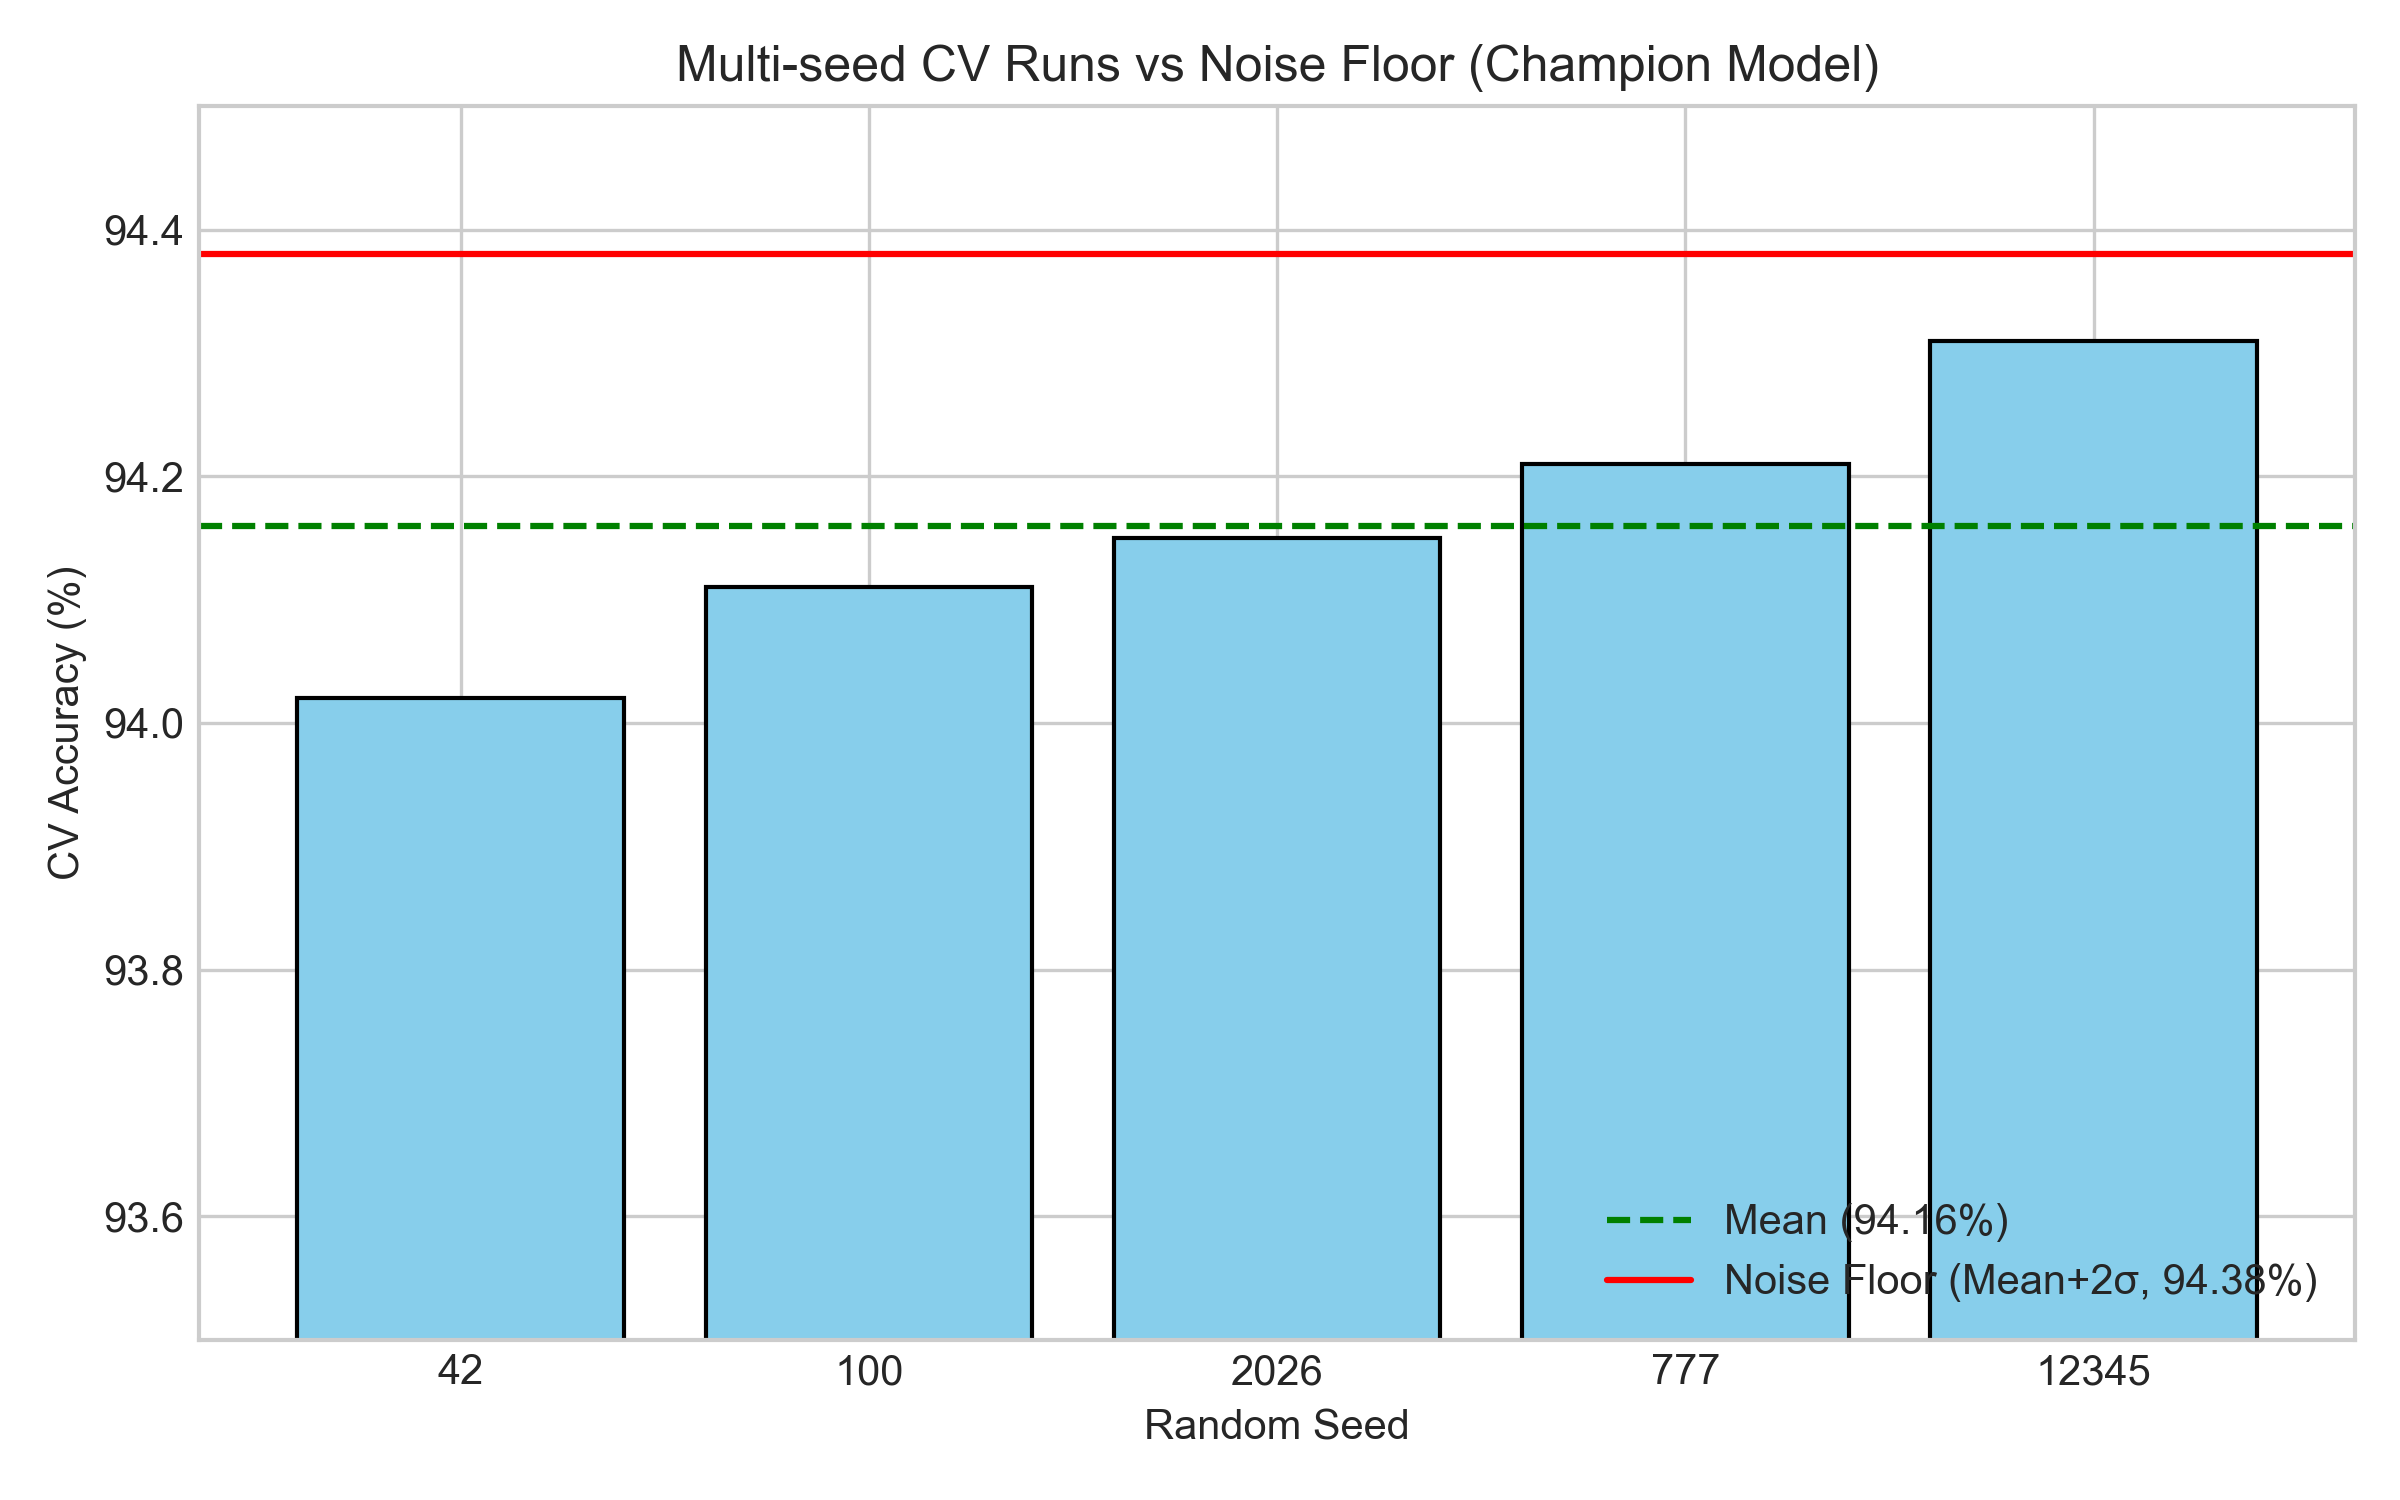
\includegraphics[width=0.55\textwidth]{plots/plot2_multiseed_noise.png}
\caption{Multi-seed CV runs vs.\ noise floor. The red line marks the $2\sigma$ acceptance threshold (94.38\%). All five seeds fall below this line, establishing the Champion baseline variance.}
\label{fig:noisefloor}
\end{figure}

% [YELLOW] Submission budget strategy
\subsection{Submission Budget Strategy}

With only 5 Kaggle submissions per day, CV was used as a triage tool and Kaggle as the scarce confirmation resource. Only models clearing the noise floor were submitted. Results were logged in an experiment log to prevent re-testing discarded configurations.

% =====================================================================
% 6. FEATURE ENGINEERING [GREEN core, YELLOW secondary]
% =====================================================================
\section{Feature Engineering}

% [GREEN] TF-IDF
\subsection{TF-IDF N-gram Features (150,000 features)}

Token-ID sequences are converted to whitespace-joined strings and vectorized using scikit-learn's \texttt{TfidfVectorizer}: unigrams through trigrams (\texttt{ngram\_range=(1,3)}), 150,000 max features, and sublinear TF ($1 + \log(\text{tf})$). This captures specific token combinations characteristic of AI vs.\ human text while dampening high-frequency tokens. Reducing the vocabulary via chi2 feature selection hurt performance; expanding to 200,000 features provided no measurable improvement. The 150,000 threshold represents the effective signal capacity.

% [YELLOW] Stylometric features
\subsection{Stylometric Features (18 features)}

Six base features (\texttt{doc\_length}, \texttt{unique\_tokens}, type-token ratio, OOV rate, Shannon entropy, zlib compression ratio) capture document-level distributional statistics. Twelve extended features add bigram entropy, bigram TTR, positional statistics (head/tail mean token IDs), frequency concentration (top-1 and top-5 relative frequency, hapax rate), and vocabulary range (token range, Q25, Q75). These features provide signal orthogonal to TF-IDF: while TF-IDF captures \textit{what} tokens are used, stylometric features capture \textit{how} the token distribution is structured. Stylometric features alone achieved ${\sim}$79.66\% CV accuracy, confirming genuine independent signal.

% [GREEN] Generative Markov features --- KEEP IN FULL, biggest result
\subsection{Generative Markov Features (8 features)}
\label{sec:gen}

This family produced the \textbf{single largest accuracy improvement} (+4.31~pp). Class-conditional bigram and trigram Markov chain transition models are built from the training data, and each document is scored by its log-likelihood under each class model.

\textbf{Implementation}: Transition counts use \textit{Python dictionaries} (not dense $V{\times}V$ matrices, which would require ${\sim}$1.3\,GB for bigrams and ${\sim}$24\,TB for trigrams at $V{=}18{,}438$). Laplace smoothing ($\alpha{=}0.1$) is applied:
$$P(t_2|t_1) = \frac{C(t_1,t_2)+\alpha}{C(t_1)+\alpha V}$$

A \textbf{Leave-One-Out (LOO)} correction subtracts each training document's own contribution to the transition counts before scoring, preventing self-memorization in $O(\text{len}(\text{doc}))$ per document.

The eight features are: \texttt{ll\_human\_bi}, \texttt{ll\_ai\_bi}, \texttt{ll\_diff\_bi} (human$-$machine; the most discriminative signal), their trigram counterparts, Zipf slope, and mean burstiness. The log-likelihood difference features directly quantify which generative model better explains a document's transitions, capturing the fundamental difference between irregular human word choices and LLMs' statistically smooth sampling.

% [GREEN] Heaps' Law Feature
\subsection{Heaps' Law Feature (1 feature)}

The vocabulary-growth exponent $\beta$ (from $V \propto N^{\beta}$) is estimated by log-log regression over ${\sim}$20 sampled points. Humans introduce vocabulary irregularly (in bursts driven by topic shifts); LLMs exhibit smoother, more predictable growth curves.

% INCLUDE Plot 11: Heaps' Law curve
\begin{figure}[h!]
\centering
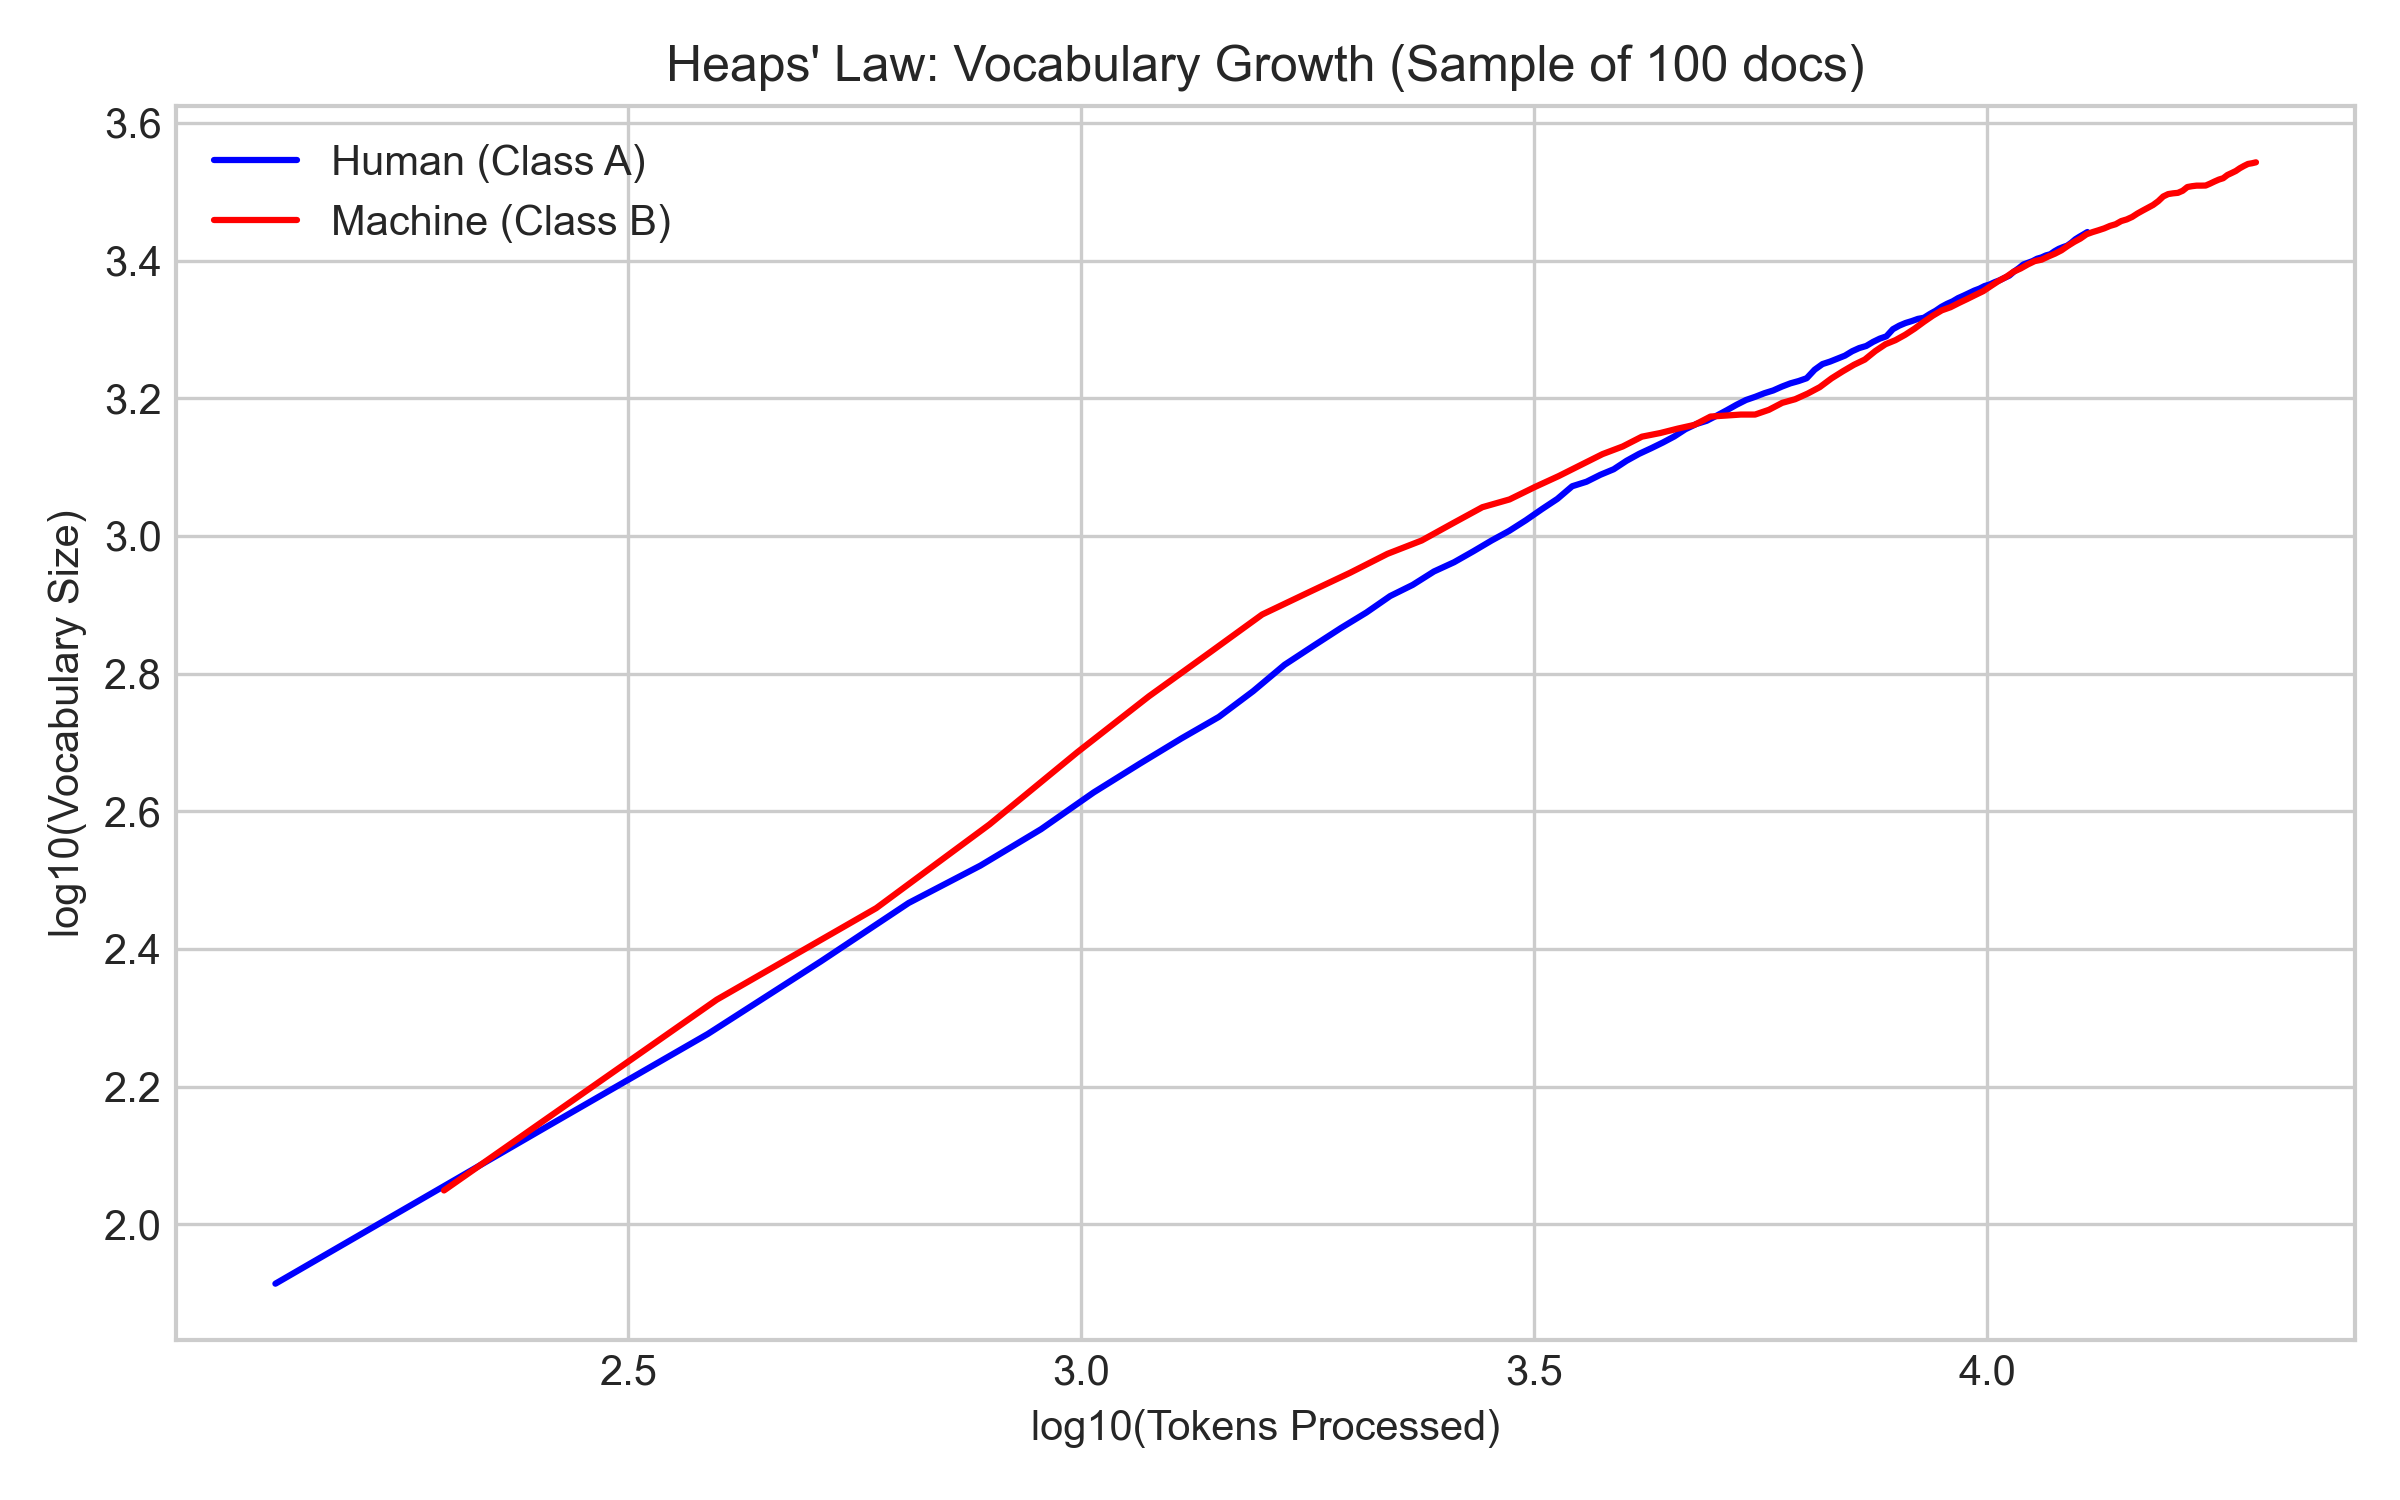
\includegraphics[width=0.55\textwidth]{plots/plot11_heaps_law.png}
\caption{Heaps' Law vocabulary growth curves (log-log scale). Machine text (red) shows smoother, more predictable vocabulary growth compared to human text (blue).}
\label{fig:heaps}
\end{figure}

% [YELLOW] Rejected features
\subsection{Features Tested and Rejected}

The following features were systematically tested against the Champion baseline using leak-free CV and the noise-floor methodology. None cleared the 94.38\% acceptance threshold:

\begin{table}[h!]
\centering
\caption{Post-noise-floor feature experiments (Champion baseline CV: 94.15\%).}
\label{tab:rejected}
\small
\begin{tabular}{@{}lccc@{}}
\toprule
\textbf{Feature Added} & \textbf{CV Acc} & \textbf{$\Delta$ vs.\ Base} & \textbf{Pass?} \\
\midrule
4th-order Quadgram & 94.20\% & +0.05 & No \\
Token Shape Stats & 94.12\% & $-$0.03 & No \\
Sliding Entropy & 94.17\% & +0.02 & No \\
Burstiness & 94.21\% & +0.06 & No \\
Graph Topology & 94.26\% & +0.11 & No \\
TF-IDF 200k & $\sim$94.22\% & +0.07 & No \\
\bottomrule
\end{tabular}
\end{table}

% [YELLOW] Feature saturation interpretation
This confirms that the Champion's 150,027 features \textit{saturate} the discriminative signal available through token-level analysis. Each new feature family was either redundant or introduced noise.

% =====================================================================
% 7. MODELS [GREEN LightGBM + Stacking, YELLOW LR/SVC, RED XGBoost]
% =====================================================================
\section{Models}

% [GREEN] LightGBM
\textbf{LightGBM} (primary): 500 trees, $\text{lr}{=}0.05$, 63 leaves, \texttt{scale\_pos\_weight}{=}1.848, L1/L2 regularization ($\alpha{=}\lambda{=}0.1$), 80\% row/column subsampling. Selected for efficient handling of sparse, high-dimensional matrices; histogram-based splitting naturally ignores zero-valued features. Systematic \textbf{hyperparameter tuning} via Optuna was attempted but terminated due to excessive runtime on the 150k-dimensional sparse matrix; robust default parameters were maintained.

% [YELLOW] Linear models
\textbf{Logistic Regression}: SAGA solver, $C{=}1.0$, balanced weights. Used as BL1 baseline and as the meta-learner in stacking ensembles.
\textbf{LinearSVC}: $C{=}0.1$, isotonic calibration (3-fold). Alternative linear baseline.

% [RED] XGBoost
\textbf{XGBoost}: 500 trees, $\text{lr}{=}0.05$, $\texttt{max\_depth}{=}6$, $\texttt{scale\_pos\_weight}{=}1.848$. Used as BL2 alternative; too slow on 150k sparse features for later experiments.

% [GREEN] Stacking
\textbf{Stacking Ensemble (Phase~B)}: OOF probabilities from Champion LightGBM + Logistic Regression $\to$ LR meta-learner with \textbf{classification threshold optimization} (0.45 instead of default 0.5). CV Accuracy: 94.22\%. \textbf{Kaggle: 96.00\%} --- tied the Champion single model.

% =====================================================================
% 8. EXPERIMENTS [GREEN core, YELLOW supporting]
% =====================================================================
\section{Experimental Results}

All experiments use 5-fold Stratified K-Fold CV (\texttt{seed=42}). Feature extractors are fit per-fold to prevent leakage.

% [GREEN] Baseline establishment
\subsection{Baseline Progression}

% **INCONSISTENCY FLAG**: The BL1/BL2 accuracy numbers below come from the user-pasted
% train.py output. SUMMARY.md shows different numbers (BL1-LogReg = 90.19%, BL2 = 89.85%)
% which likely reflect an earlier code version with different stylometric feature counts
% (10 vs 6). The numbers below correspond to the FINAL codebase (6 base StyleFeatures).

\begin{table}[h!]
\centering
\caption{Cross-validation results for baseline models.}
\label{tab:baselines}
\small
\begin{tabular}{@{}llccccc@{}}
\toprule
\textbf{Model} & \textbf{Features} & \textbf{Dim.} & \textbf{Acc} & $\pm$ & \textbf{F1} & \textbf{AUC} \\
\midrule
BL1-LogReg & TF-IDF & 150k & 0.8162 & 0.0075 & 0.8537 & 0.8984 \\
BL1-SVC & TF-IDF & 150k & 0.8054 & 0.0084 & 0.8406 & 0.8838 \\
BL2-LGBM & Stylometric & 6 & 0.7966 & 0.0056 & 0.8506 & 0.8711 \\
BL2-XGB & Stylometric & 6 & 0.7986 & 0.0069 & 0.8541 & 0.8786 \\
BL3-Combined & TF-IDF+Style & 150,006 & 0.8982 & 0.0110 & 0.9183 & 0.9654 \\
BL3b-Generative & +ExtStyle+Gen & 150,026 & \textbf{0.9413} & 0.0058 & 0.9543 & 0.9833 \\
BL4-Ensemble & OOF Stack (6) & 6 & 0.9424 & --- & 0.9550 & 0.9812 \\
\bottomrule
\end{tabular}
\end{table}

% [GREEN] Key observations
\textbf{Key observations}: (1)~Stylometric features alone (BL2, 6~features) achieve ${\sim}$80\%, proving genuine structural signal without vocabulary. (2)~Combining TF-IDF with style features (BL3) jumps to 89.82\% (+8.2~pp). (3)~Adding generative Markov features (BL3b) produces a \textbf{+4.31~pp} gain---the largest single improvement. (4)~The stacking ensemble (BL4) provides only marginal improvement over BL3b (94.24\% vs.\ 94.13\%), suggesting BL3b already captures most ensemble diversity.

% INCLUDE Plot 7: Confusion Matrix
\begin{figure}[h!]
\centering
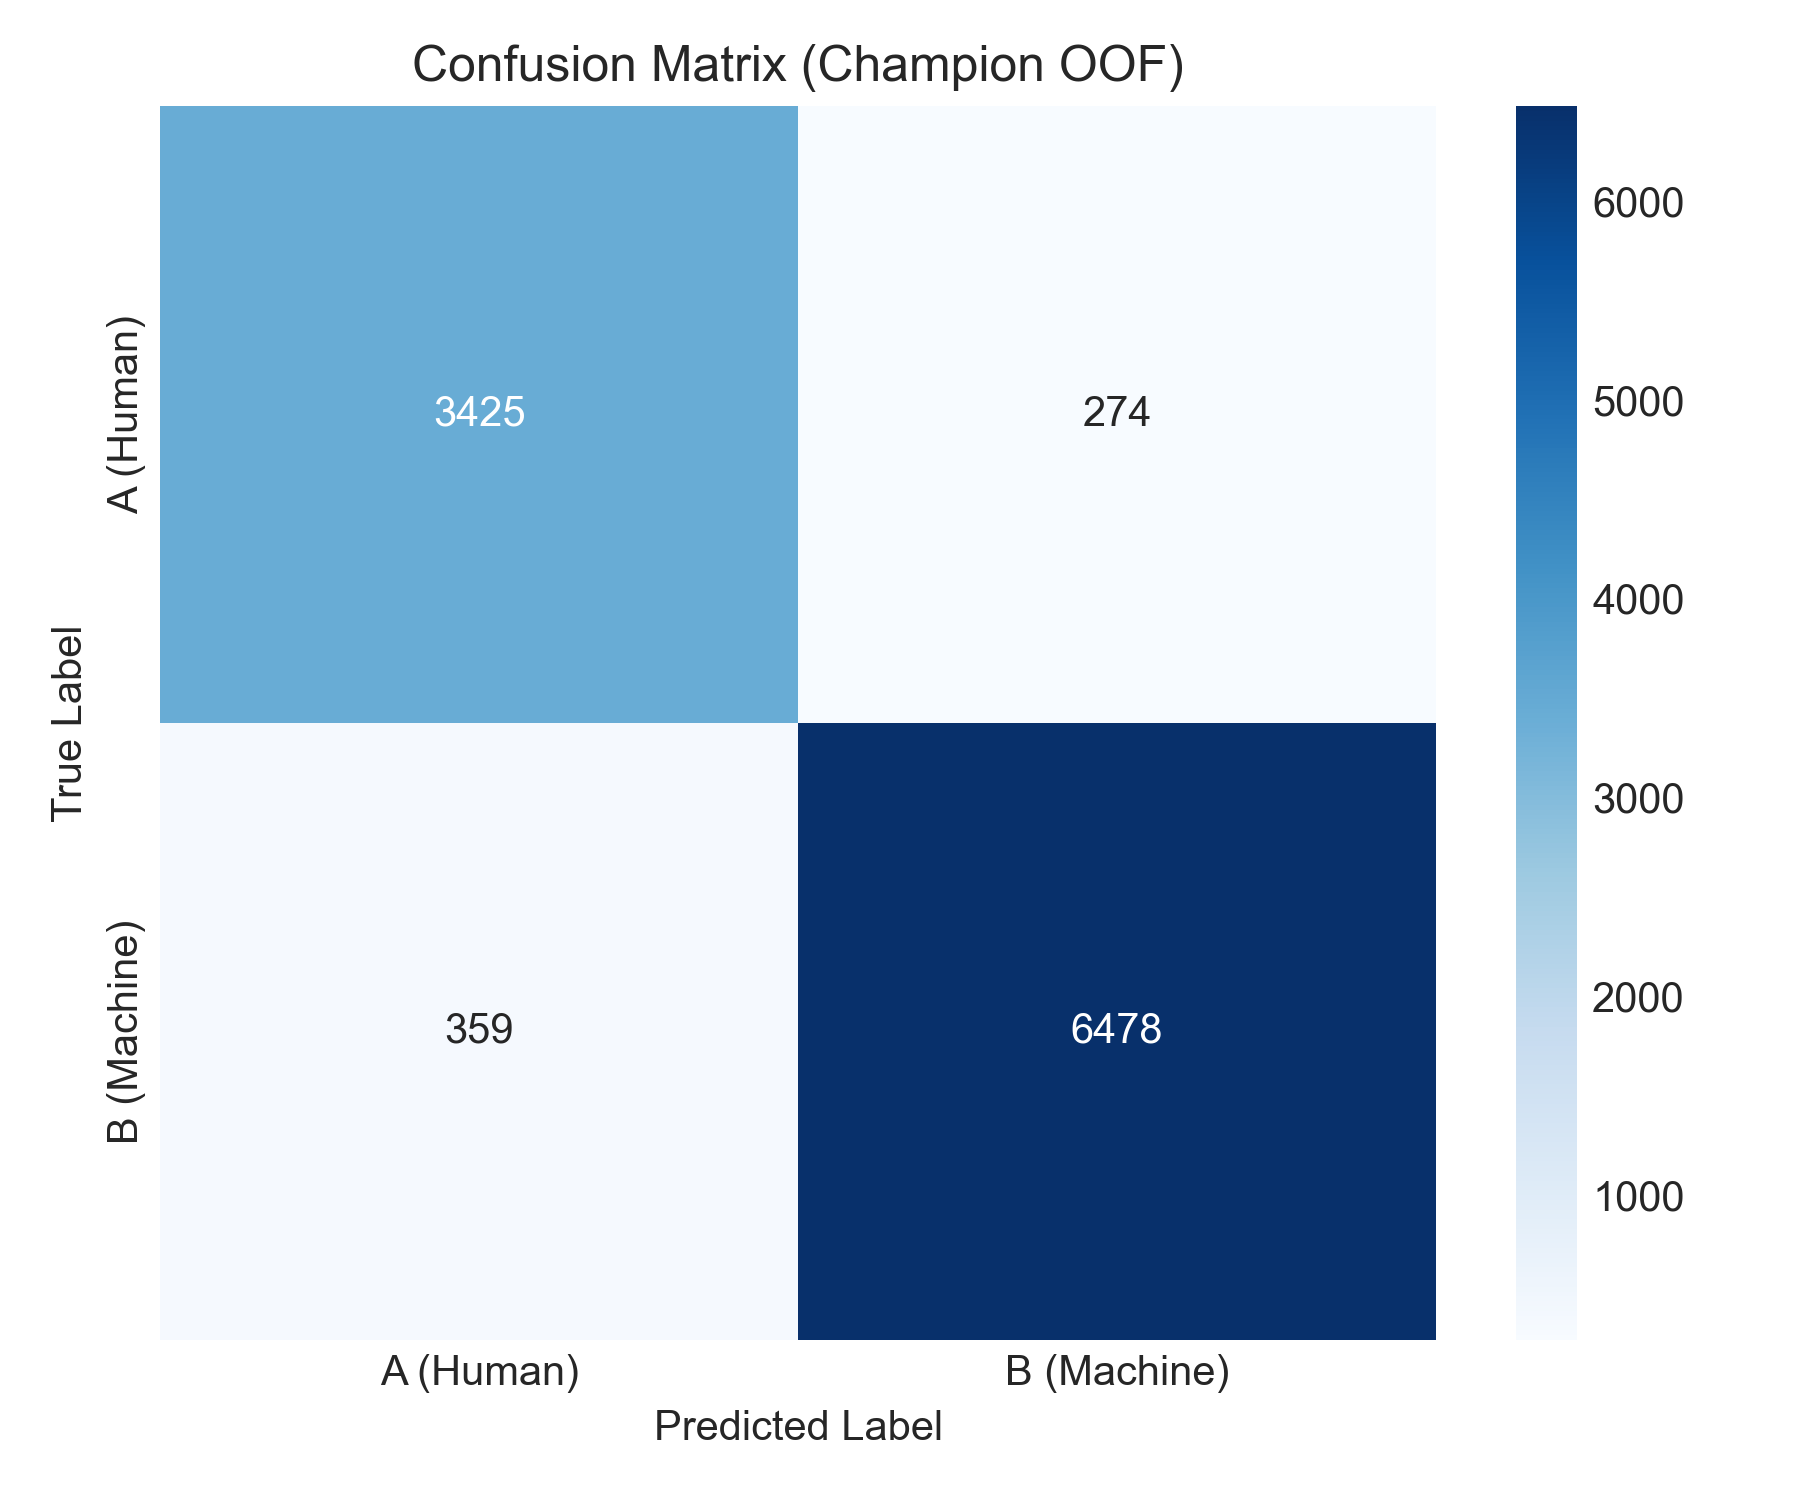
\includegraphics[width=0.45\textwidth]{plots/plot7_confusion_matrix.png}
\caption{Confusion matrix (Champion OOF predictions, threshold 0.5). The model misclassifies 274 human documents as machine and 359 machine documents as human.}
\label{fig:confusion}
\end{figure}

% [GREEN] Champion model and noise floor
\subsection{Champion Model and Noise-Floor Establishment}

Adding the Heaps' Law feature to BL3b yields the \textbf{Champion} (150,027 features). Multi-seed CV (seeds 42, 100, 2026, 777, 12345) established a noise floor of $94.15\% \pm 0.12\%$, giving a $2\sigma$ acceptance threshold of \textbf{94.38\%}. \textbf{Kaggle: 96.00\%} (confirmed across three independent submissions).

% [GREEN] Leak-free CV revalidation
Early standalone scripts fitted TF-IDF on the full training set before CV splitting (acknowledged data leakage). Leak-free replication confirmed $\sim$0.4\% CV inflation from this leakage, but it only affected internal CV estimates---Kaggle submissions were unaffected since the final training step uses all training data.

% [YELLOW] Dimensionality reduction
\subsection{Dimensionality Reduction}

Compressing 150k TF-IDF features to 300 via TruncatedSVD reduced CV accuracy from 94.62\% to 94.41\%. Sparse exact n-gram matches encode highly specific lexical fingerprints that are blurred by dimensionality reduction. LightGBM already handles sparse matrices efficiently by not splitting on zero-valued features, making explicit dimensionality reduction counterproductive.

% [GREEN] Phase B stacking
\subsection{Phase~B Stacking Ensemble}

% INCLUDE Plot 8: Threshold sweep
OOF stacking of Champion LightGBM + Logistic Regression $\to$ LR meta-learner, with threshold optimization. Figure~\ref{fig:threshold} shows the threshold sweep: the optimal threshold of 0.45 maximizes OOF accuracy. Result: 94.22\% CV / \textbf{96.00\% Kaggle} --- tied the Champion single model.

\begin{figure}[h!]
\centering
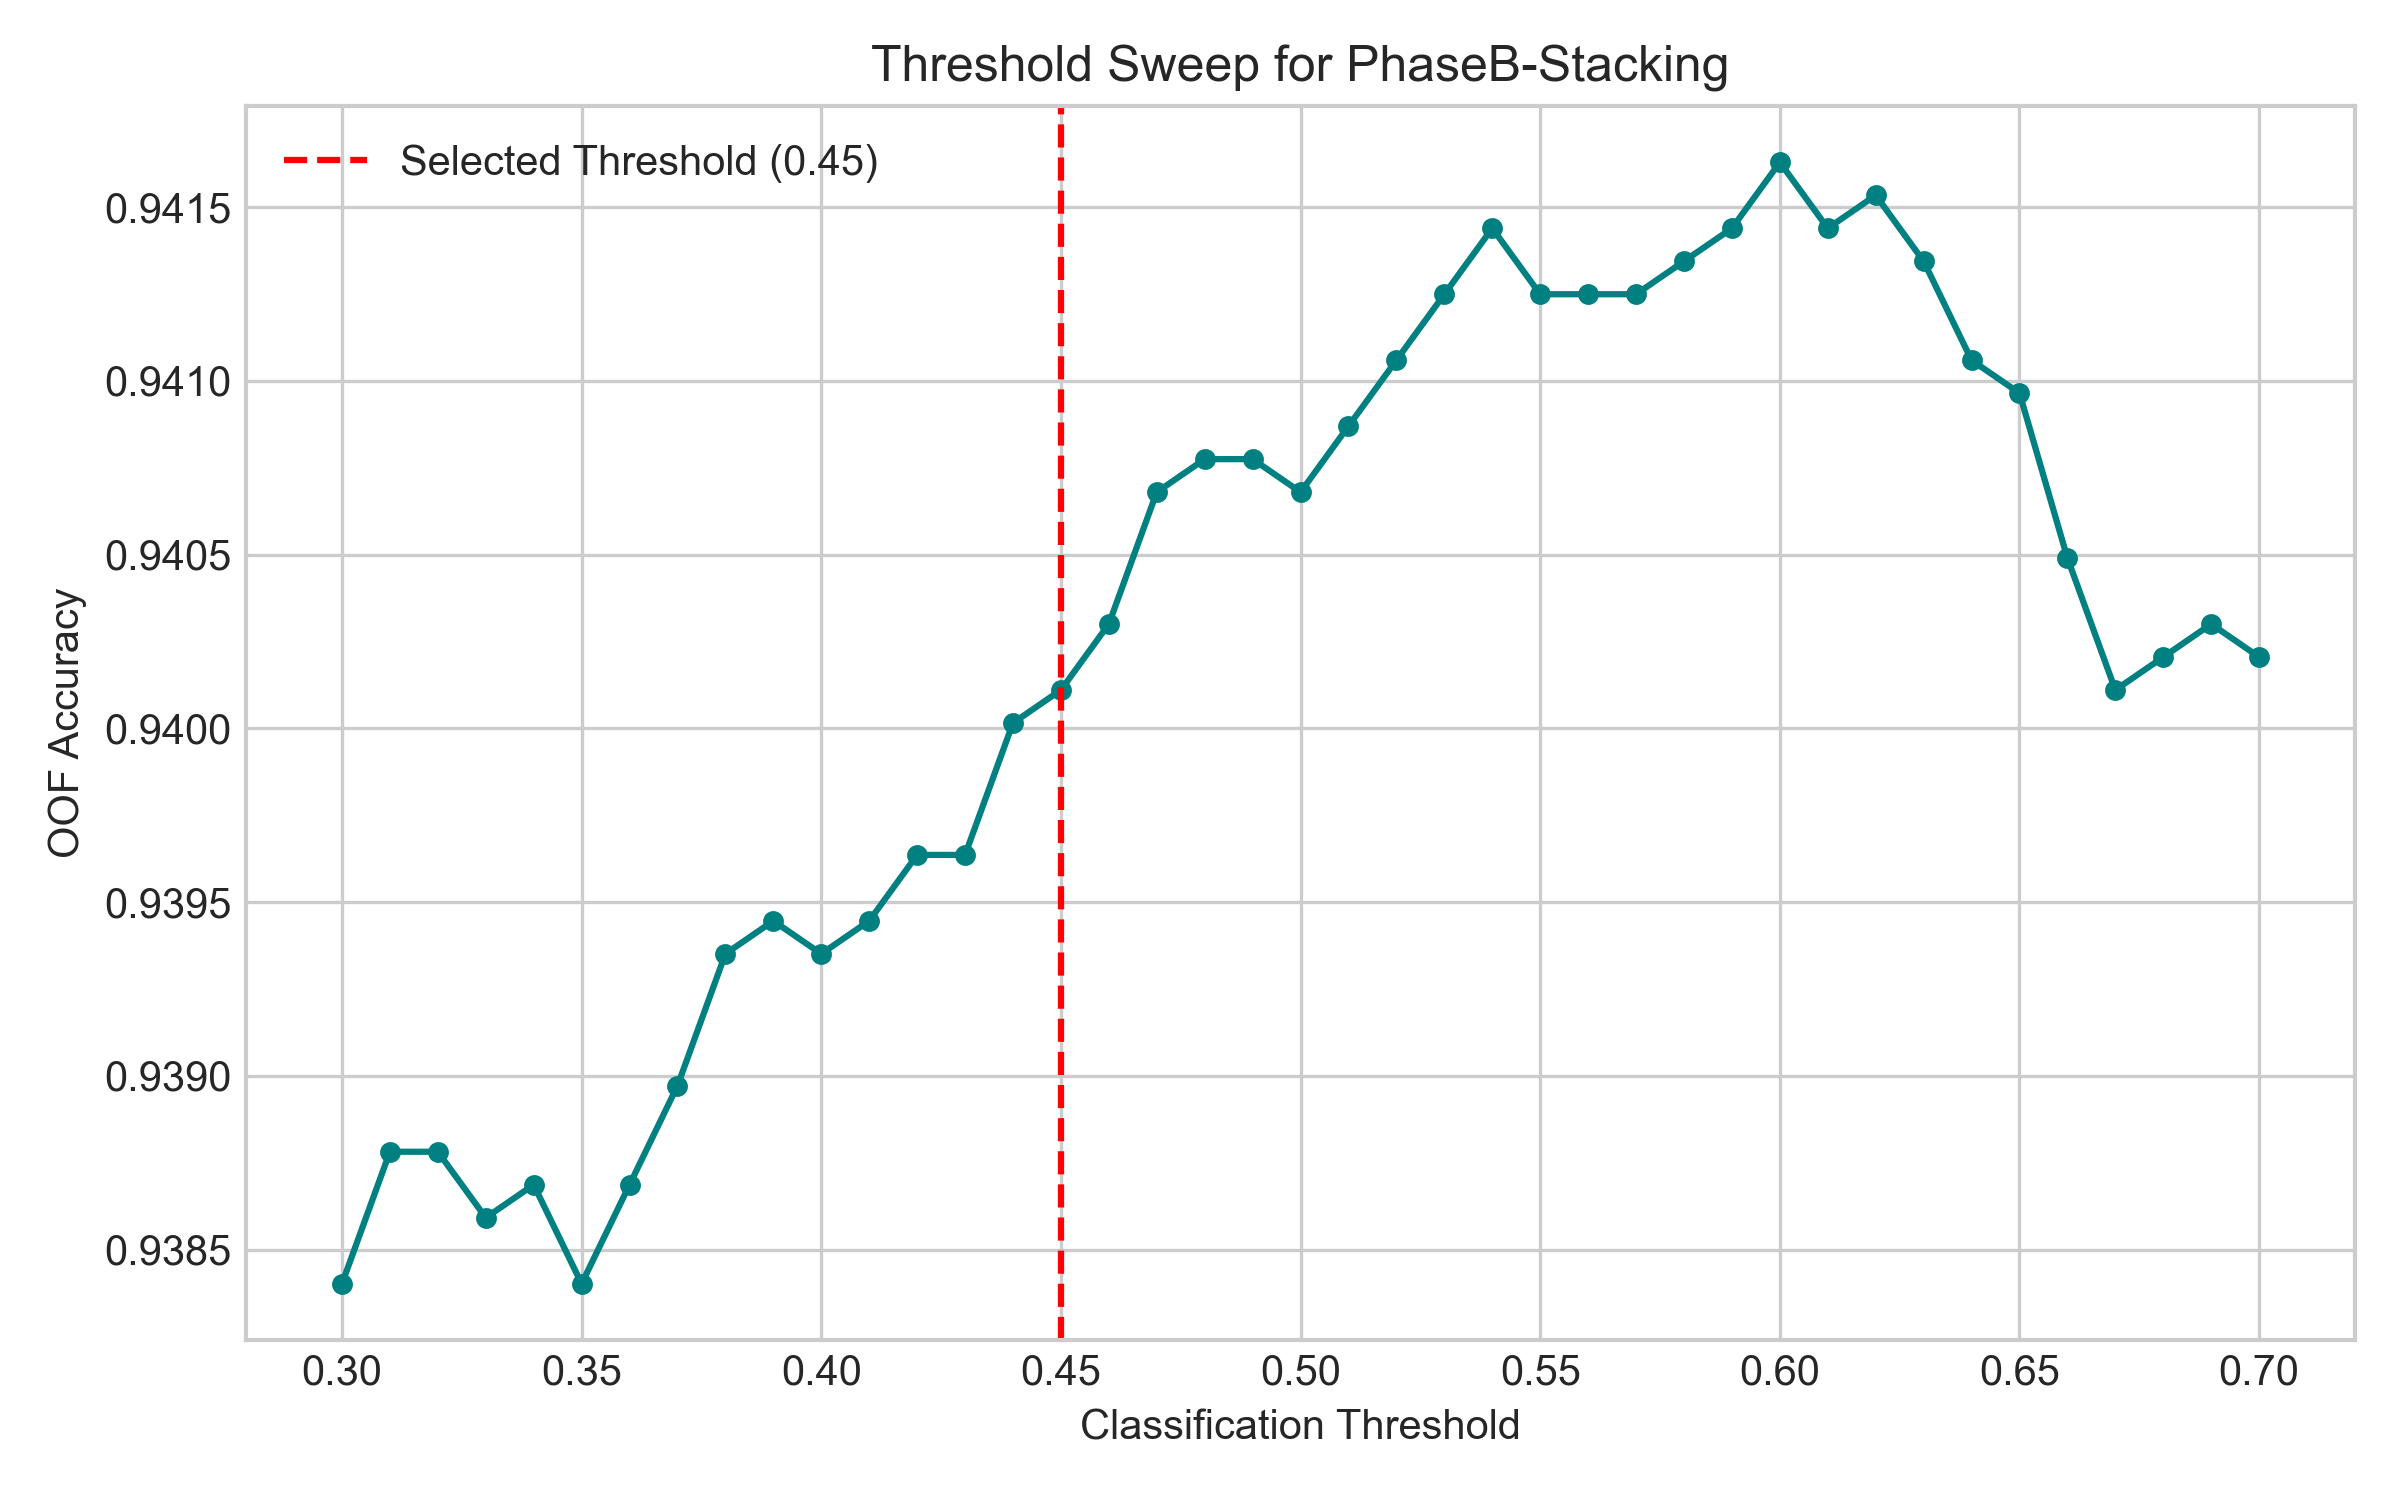
\includegraphics[width=0.55\textwidth]{plots/plot8_threshold_sweep.png}
\caption{Classification threshold sweep for Phase~B stacking. The selected threshold (0.45, red dashed) shifts the decision boundary to account for class imbalance.}
\label{fig:threshold}
\end{figure}

% INCLUDE Plot 6: ROC Curve
\begin{figure}[h!]
\centering
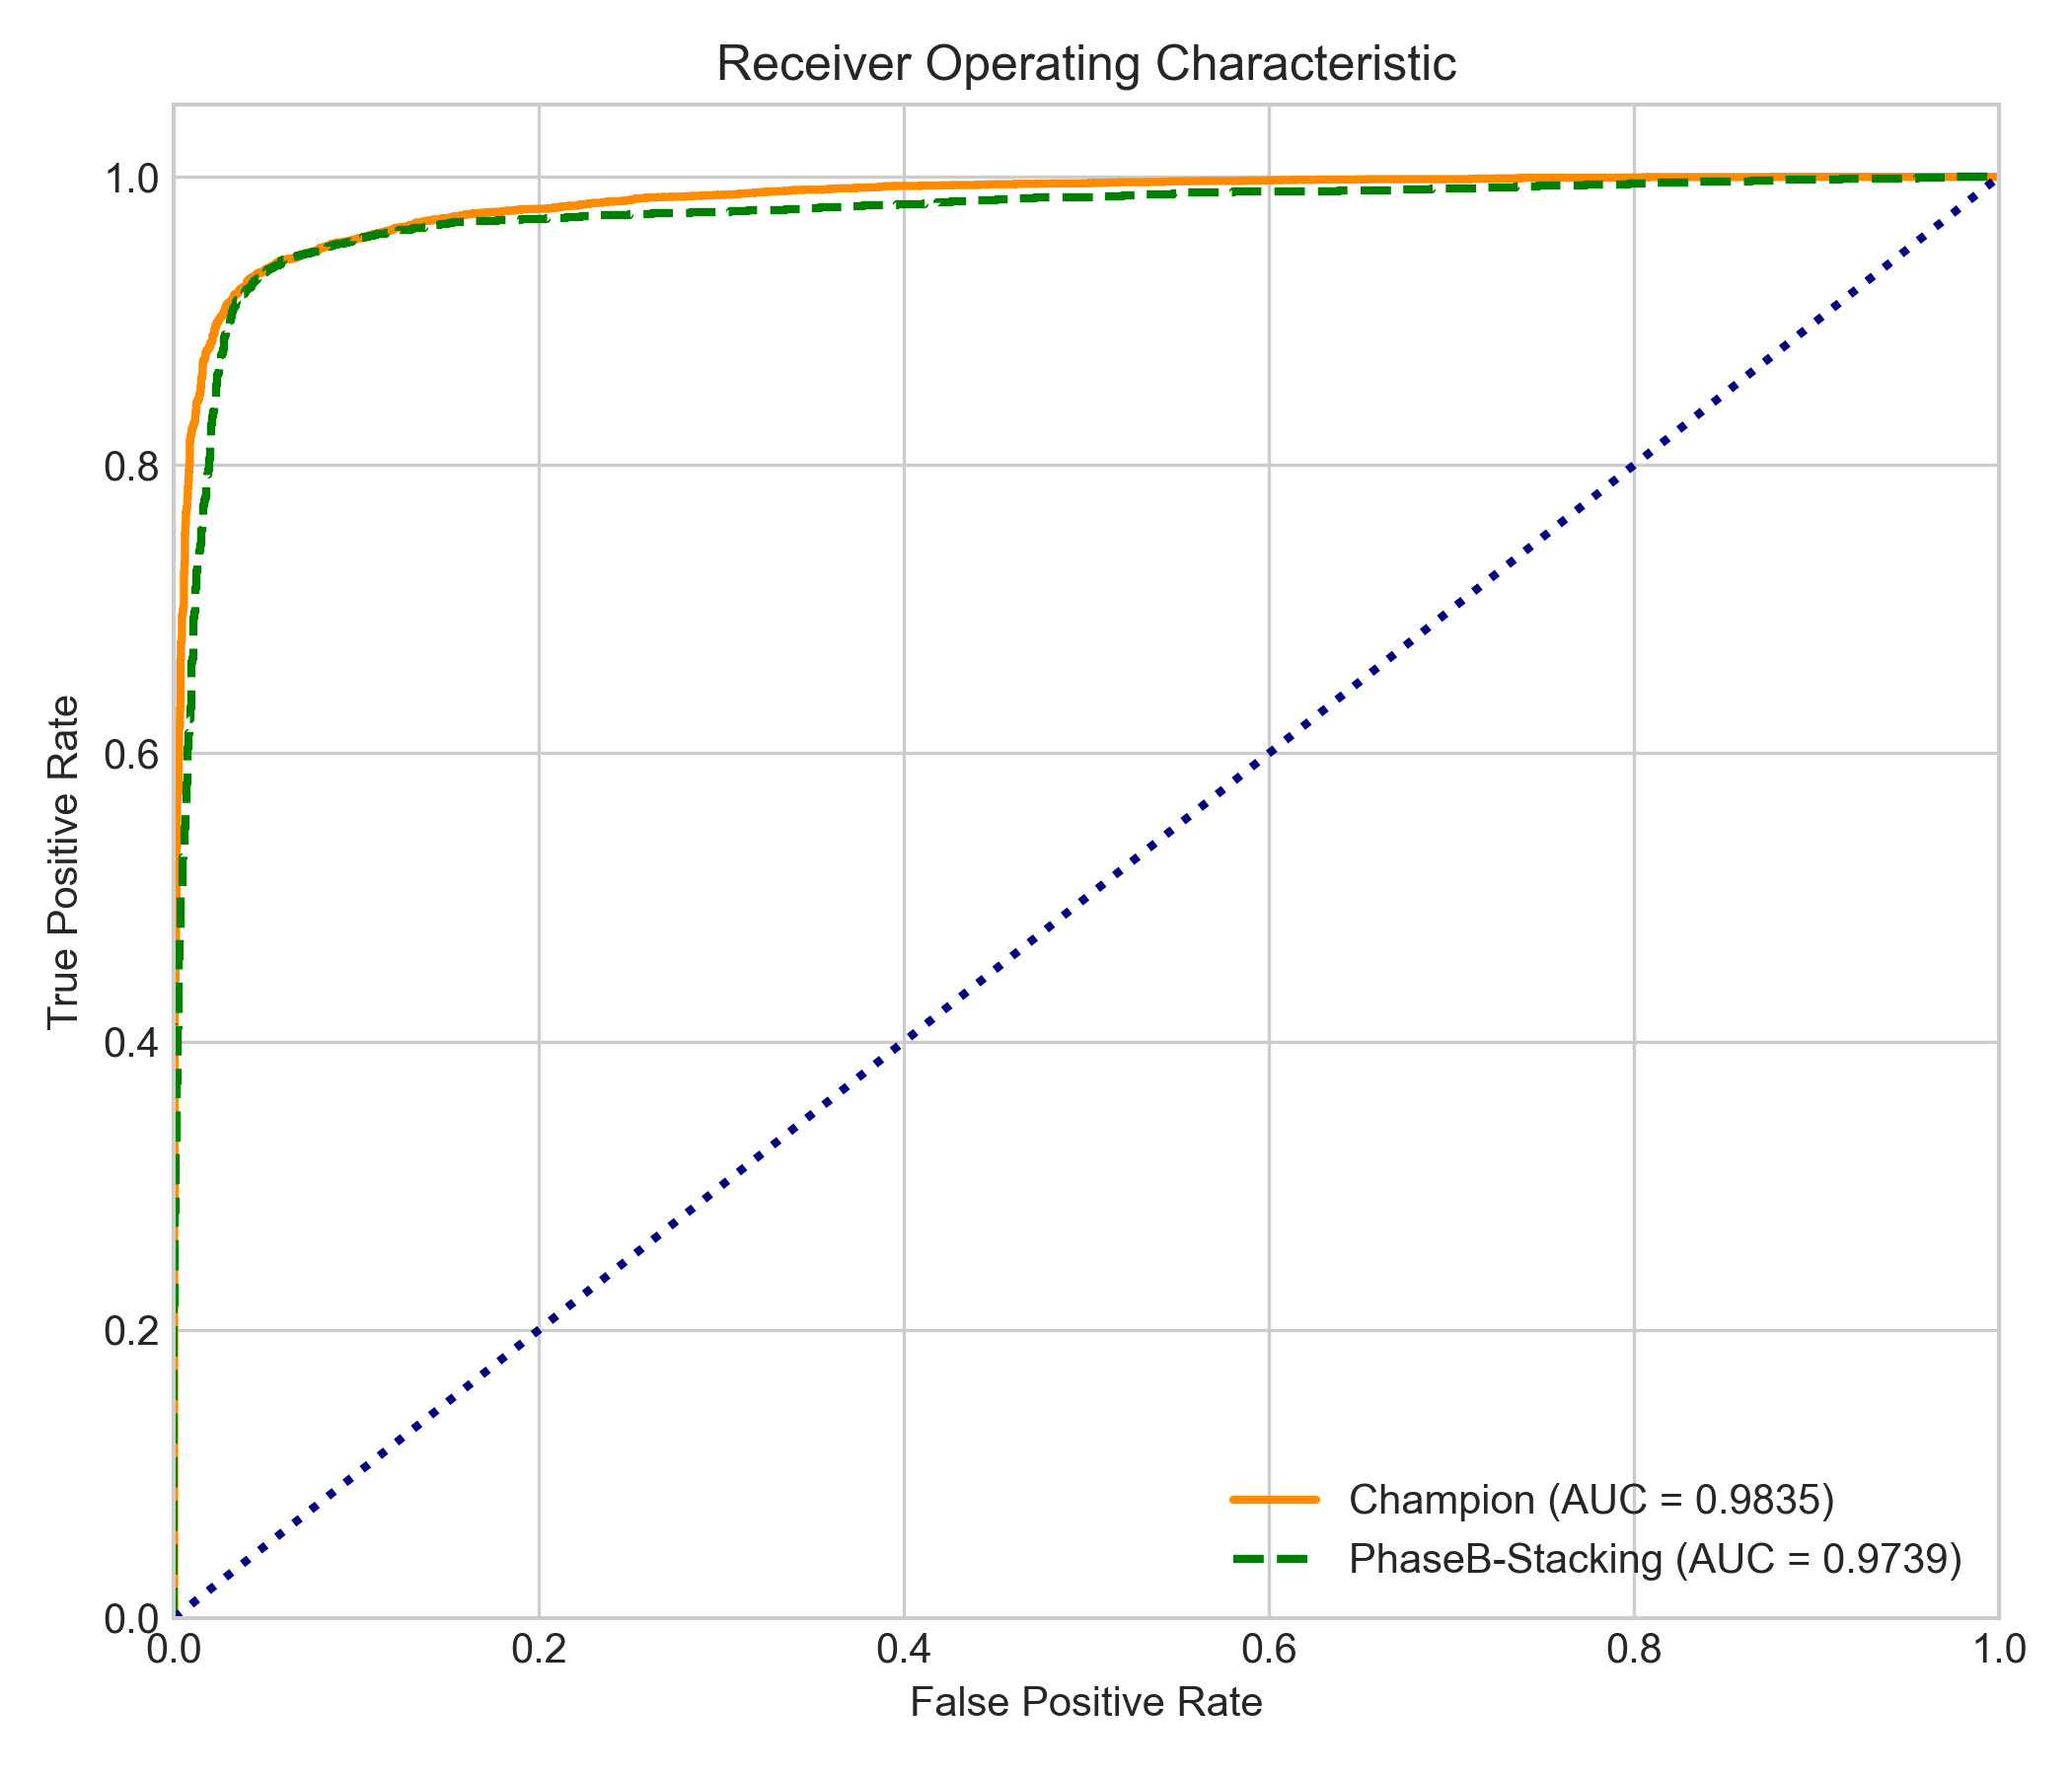
\includegraphics[width=0.50\textwidth]{plots/plot6_roc_curve.png}
\caption{ROC curves for Champion LightGBM (AUC = 0.9835) and Phase~B Stacking ensemble (AUC = 0.9739). Both achieve near-identical discrimination.}
\label{fig:roc}
\end{figure}

% [YELLOW] Pseudo-labeling
\subsection{Pseudo-Labeling}

Two independent attempts at self-training with high-confidence test predictions:

\begin{table}[h!]
\centering
\caption{Pseudo-labeling experiments (Champion Kaggle baseline: 96.00\%).}
\label{tab:pseudo}
\small
\begin{tabular}{@{}lcccc@{}}
\toprule
\textbf{Attempt} & \textbf{Threshold} & \textbf{CV Acc} & \textbf{Kaggle} & \textbf{Decision} \\
\midrule
Attempt 1 & 0.95 / 0.05 & 94.92\%$^*$ & 94.86\% & Rejected \\
Attempt 2 & 0.98 / 0.02 & 94.58\% & 95.53\% & Rejected \\
\bottomrule
\end{tabular}
\begin{flushleft}
\scriptsize $^*$CV estimate includes TF-IDF leakage (inflated by ${\sim}$0.4~pp).
\end{flushleft}
\end{table}

Both attempts inflated CV while \textit{degrading} Kaggle performance. The mechanism: self-training reinforces the model's existing confident predictions on easy examples (deepening decision boundaries) without improving classification of ambiguous edge-cases. The model's own highest-confidence guesses are fed back as ground truth, creating a self-reinforcing echo chamber. Pseudo-labeling was retired.

% [GREEN] Kaggle Leaderboard Summary
\subsection{Kaggle Leaderboard Summary}

\begin{table}[h!]
\centering
\caption{All Kaggle submissions.}
\label{tab:kaggle}
\small
\begin{tabular}{@{}lcc@{}}
\toprule
\textbf{Configuration} & \textbf{CV Acc} & \textbf{Kaggle} \\
\midrule
Champion LightGBM (150,027 feat.) & 94.15\% & \textbf{96.00\%} \\
Champion (leak-free replication) & 94.18\% & \textbf{96.00\%} \\
Phase B Stacking (threshold 0.45) & 94.22\% & \textbf{96.00\%} \\
Phase 4 Pseudo-Labeling & 94.58\% & 95.53\% \\
Ultimate Model (all + pseudo) & 95.00\%$^*$ & 94.86\% \\
\bottomrule
\end{tabular}
\end{table}

% [GREEN] Feature ablation summary
\textbf{Feature ablation summary}: TF-IDF alone (BL1): 81.62\% $\to$ +Stylometric (BL3): 89.82\% (+8.20~pp) $\to$ +Generative (BL3b): 94.13\% (+4.31~pp) $\to$ +Heaps' Law (Champion): 94.18\% (+0.05~pp, leak-free). Kaggle: 96.00\%.

% INCLUDE Plot 9: Feature Importance
\begin{figure}[h!]
\centering
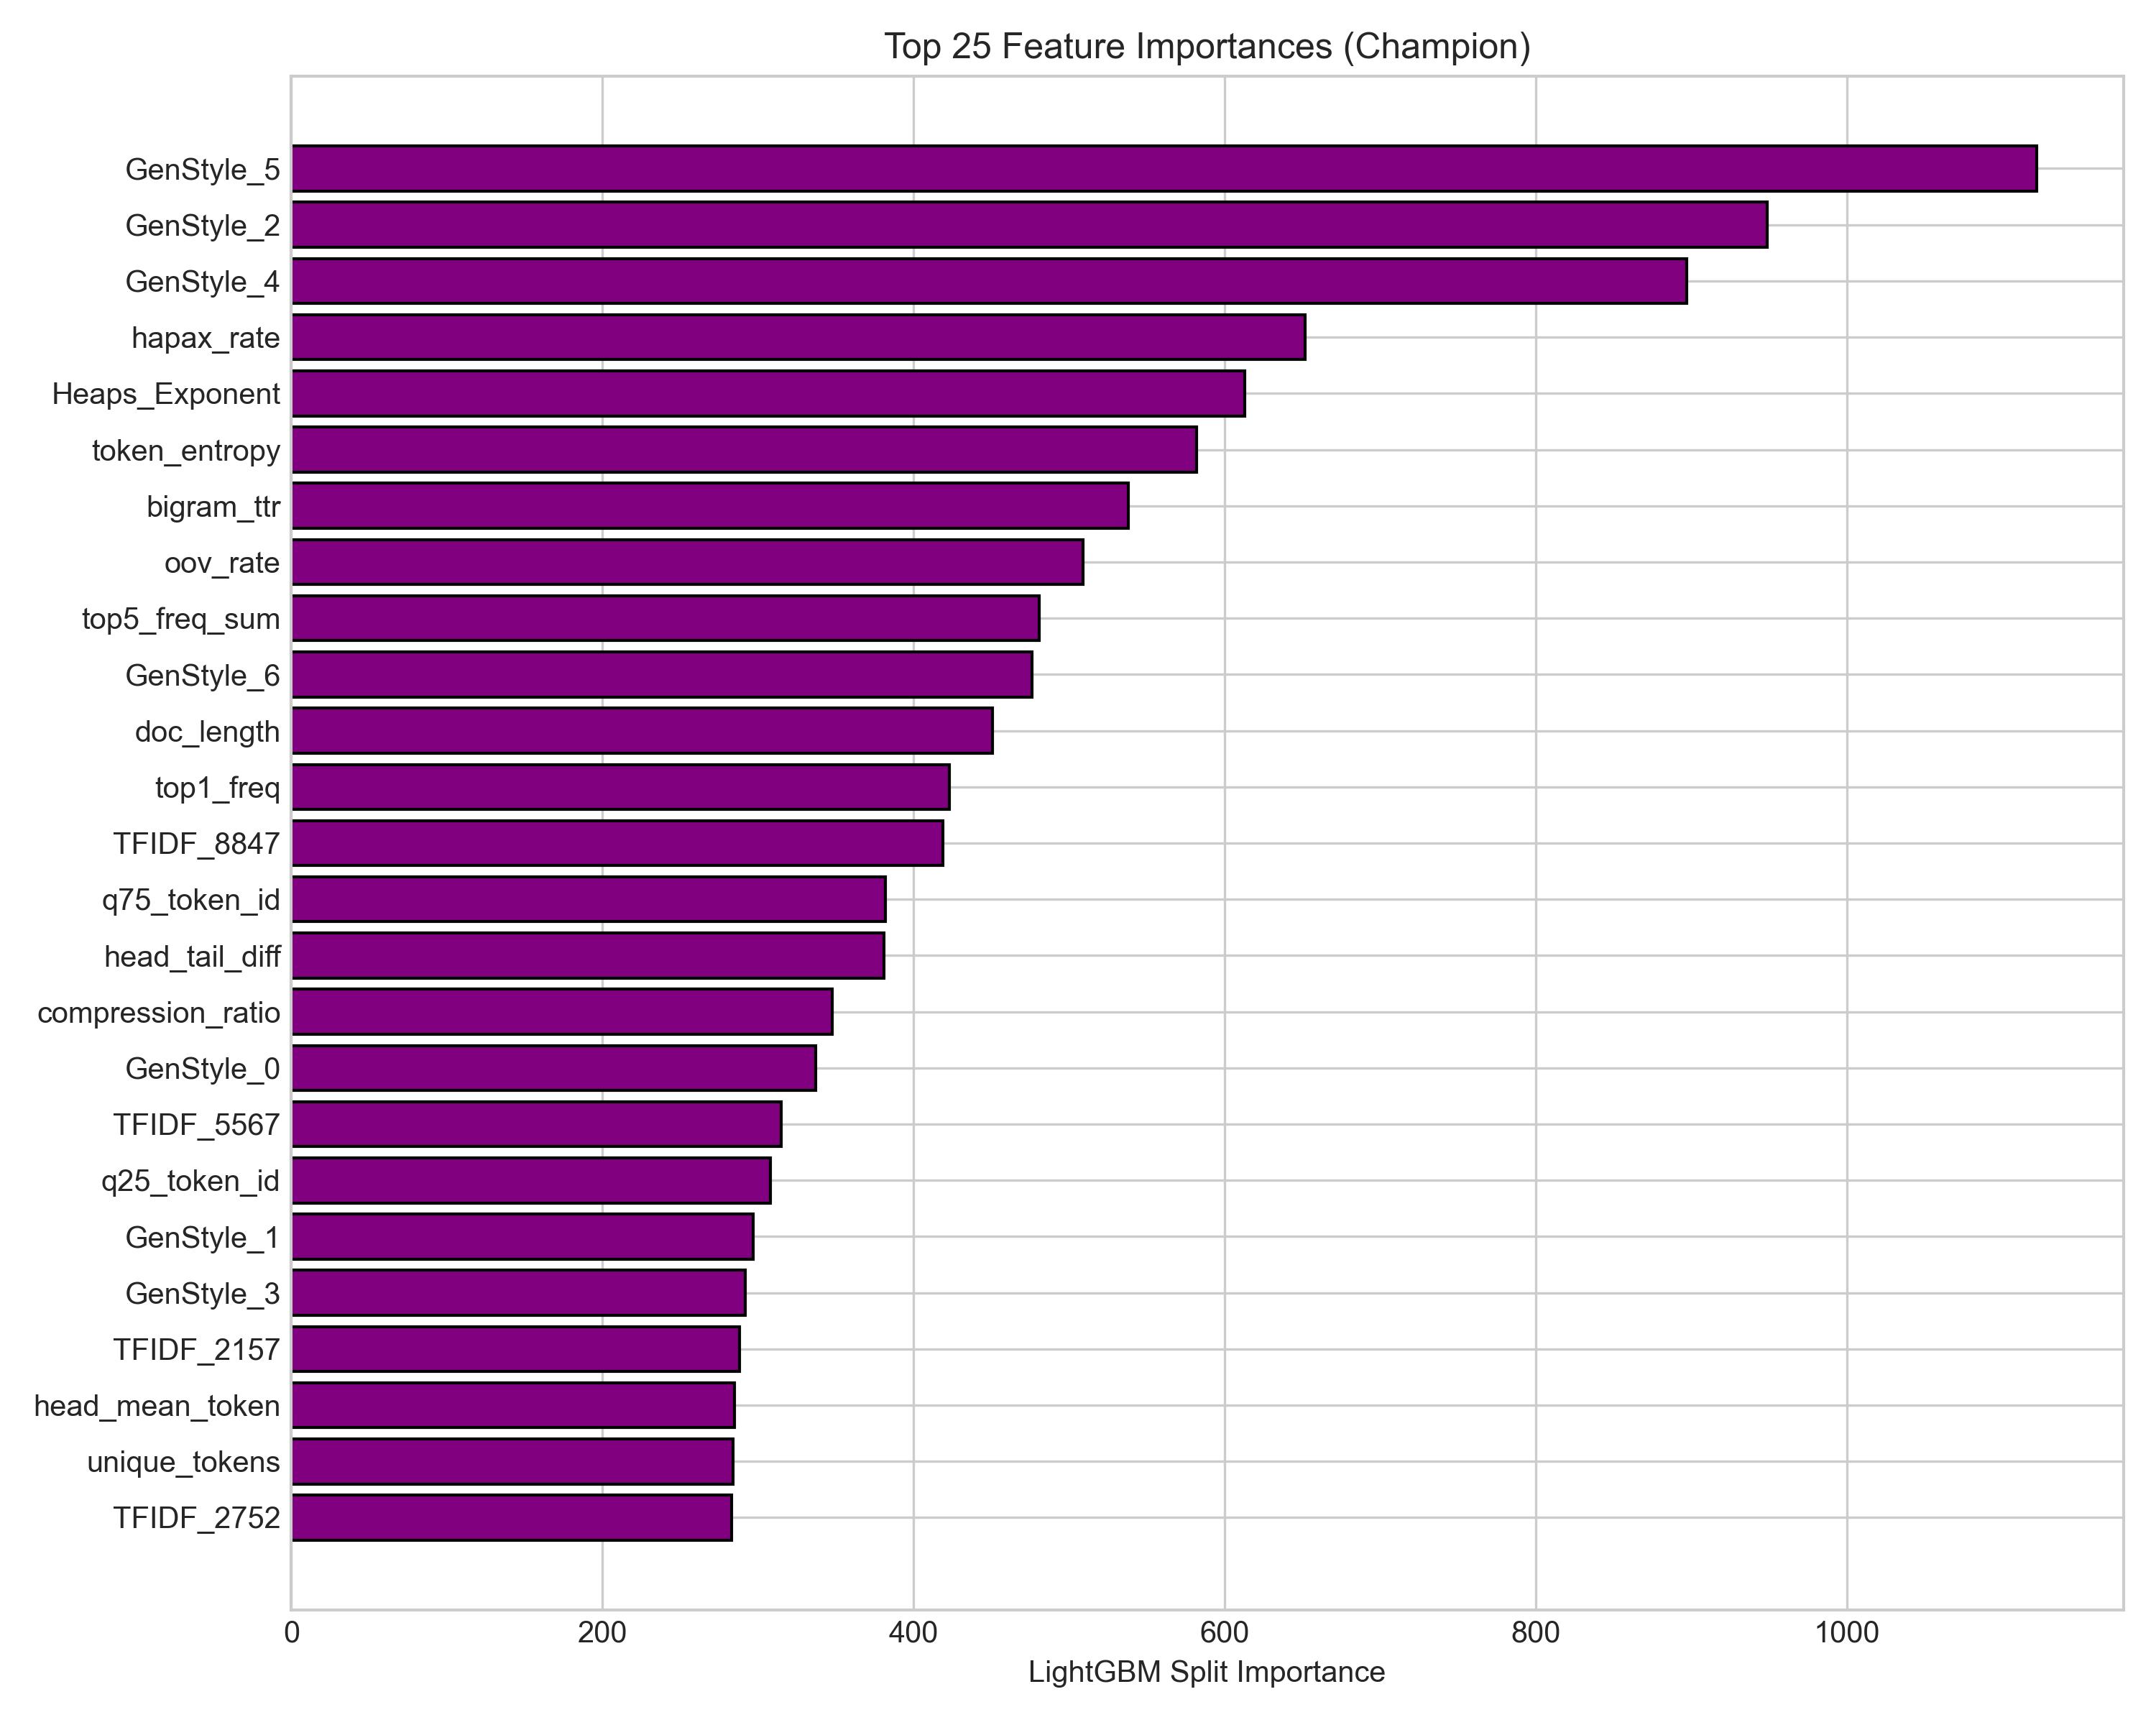
\includegraphics[width=0.60\textwidth]{plots/plot9_feature_importance.png}
\caption{Top 25 LightGBM feature importances (split count). Generative features (\texttt{GenStyle\_5}, \texttt{GenStyle\_2}, \texttt{GenStyle\_4}) dominate, followed by stylometric features (\texttt{hapax\_rate}, \texttt{Heaps\_Exponent}, \texttt{token\_entropy}). TF-IDF features appear individually only in the lower ranks, reflecting their collective rather than individual contribution.}
\label{fig:importance}
\end{figure}

% =====================================================================
% 10. DISCUSSION [GREEN core, YELLOW secondary]
% =====================================================================
\section{Discussion}

% [GREEN] Why TF-IDF works
\textbf{Why TF-IDF provides a strong base signal.}
Token n-grams capture specific vocabulary patterns that differ between human and machine text. Sublinear TF dampens common tokens, giving weight to rarer but more discriminative n-grams. Even without raw words, the statistical distribution of token-ID n-grams is highly discriminative (81.62\% with a linear model).

% [GREEN] The Generative Feature Breakthrough
\textbf{The generative feature breakthrough (+4.31~pp).}
Standard TF-IDF captures token \textit{frequencies} but discards sequential dependency. The Markov features recover this by computing the probability of token \textit{sequences} under class-conditional models. The log-likelihood difference (\texttt{ll\_diff}) directly quantifies which generative model better explains a document's transitions---the single most informative derived signal (Figure~\ref{fig:importance}).

% [GREEN] Stylometric independence
\textbf{Why stylometric features work without raw words.}
Even on integer token IDs, distributional statistics (entropy, compression ratio, TTR) capture structural properties. These are orthogonal to TF-IDF: TF-IDF captures \textit{what} is said; stylometrics capture \textit{how} it is structured. BL2's ${\sim}$80\% accuracy on stylometrics alone confirms genuine independent signal.

% [GREEN] CV/LB gap
\textbf{The CV/Leaderboard gap.}
A consistent ${\sim}$1.8~pp gap between leak-free CV (${\sim}$94.15\%) and Kaggle (96.00\%) was observed across all three independently submitted configurations. This gap made CV unreliable as an absolute predictor of leaderboard performance, although relative ordering was generally preserved. The gap may reflect distributional differences between the training and test sets.

% [GREEN] Why pseudo-labeling failed
\textbf{Why pseudo-labeling structurally failed.}
Self-training adds the model's highest-confidence predictions back as training labels---precisely the examples it already classifies correctly with high margin. Retraining deepens existing decision boundaries without providing new information about the ambiguous boundary region. Both attempts exhibit inflated CV relative to their leaderboard performance, and both underperform the Champion model despite appearing stronger in CV.

% [YELLOW] Why SVD hurt
\textbf{Why dimensionality reduction hurt.}
TruncatedSVD blurs sharp, specific n-gram patterns into smooth ``topics,'' losing fine-grained discriminative signals. LightGBM's histogram-based splitting already handles irrelevant sparse features efficiently.

% [YELLOW] Feature saturation
\textbf{Feature saturation.}
The Phase C testing demonstrated that the Champion's 150,027 features exhaustively capture the discriminative signal accessible through token-level analysis. Six candidate extensions (quadgrams, shape stats, sliding entropy, burstiness, graph topology, vocabulary expansion) all failed to clear the noise floor.

% =====================================================================
% 11. LIMITATIONS [YELLOW --- condense to 5 bullets if trimming]
% =====================================================================
\section{Limitations}

\begin{enumerate}
% [YELLOW] --- include top 5, cut rest if space-tight
    \item \textbf{Dataset specificity}: Results are specific to this competition's tokenization and may not generalize to raw text or unseen LLMs.
    \item \textbf{CV/LB discrepancy}: The ${\sim}$1.8~pp gap makes local evaluation unreliable for fine-grained comparisons.
    \item \textbf{No systematic hyperparameter tuning}: Optuna was attempted but terminated for runtime; LightGBM uses robust defaults.
    \item \textbf{High-dimensional sparse representation}: 150k features carry overfitting risk, mitigated by LightGBM's regularization and subsampling.
    \item \textbf{Single-seed post-noise-floor tests}: While the noise floor was established with 5 seeds, individual feature tests used only seed 42.
% [RED] --- cut these first
    \item \textbf{Unknown tokenizer}: Cannot compute ``sentence length'' or ``punctuation rate'' directly.
    \item \textbf{Limited submission budget}: 5/day prevented exhaustive leaderboard validation.
    \item \textbf{Pseudo-labeling contamination risk}: Using test predictions as labels introduces systematic bias.
\end{enumerate}

% =====================================================================
% 13. BONUS MARK: CONTROLLED COMPARISON [GREEN]
% =====================================================================
\section{Bonus Mark: Controlled Comparison}

We provide a strict controlled comparison demonstrating the impact of dictionary-based generative Markov features (Section~\ref{sec:gen}).

\textbf{Control} (BL3-Combined): TF-IDF (150k) + 6 base StyleFeatures $\to$ LightGBM.\\
\textbf{CV Accuracy: 89.82\%.}

\textbf{Treatment} (BL3b-Generative): TF-IDF (150k) + 18 ExtendedStyleFeatures + 8 GenerativeStyleFeatures $\to$ LightGBM.\\
\textbf{CV Accuracy: 94.13\% (+4.31~pp).}

Both use identical validation protocol (5-fold Stratified K-Fold, seed~42), identical LightGBM hyperparameters, and identical TF-IDF configuration. The \textit{only} difference is the addition of the generative and extended features.

\textbf{Justification}: TF-IDF captures token \textit{frequencies} but discards sequential dependencies. The Markov chain features recover this by computing class-conditional transition probabilities---directly measuring whether a document's token-to-token transitions look more like human writing or LLM sampling. The dictionary-based implementation avoids the infeasible $V^2$/$V^3$ dense matrices, and the LOO correction prevents training-set self-memorization.

% =====================================================================
% 14. CONCLUSION [GREEN]
% =====================================================================
\section{Conclusion}

We developed a 150,027-feature classification pipeline achieving \textbf{96.00\% accuracy} on the Kaggle leaderboard for distinguishing human-authored from machine-generated text on pre-tokenized integer sequences. The most impactful contribution was memory-efficient, class-conditional Markov chain log-likelihood features (+4.31~pp over TF-IDF + stylometrics). A noise-floor methodology based on multi-seed CV prevented submission of statistically insignificant improvements and correctly filtered six candidate features. Two pseudo-labeling experiments provided clear evidence that self-training inflates CV without improving generalization. The combination of lexical, statistical, sequential, and information-theoretic signals saturates the discriminative capacity of token-level analysis for this dataset.

% =====================================================================
% 15. REFERENCES [RED --- include only if space]
% =====================================================================
% [RED] No papers cited in the project. Include only if space allows.
% Recommended citations if included:
% [1] Ke et al., LightGBM: A Highly Efficient Gradient Boosting Decision Tree, NeurIPS 2017.
% [2] Heaps, H.S., Information Retrieval: Computational and Theoretical Aspects, 1978.
% [3] Salton and Buckley, Term-weighting approaches in automatic text retrieval, IPM 1988.
% [4] Lee, D-H., Pseudo-Label: The Simple and Efficient Semi-Supervised Learning Method, ICML Workshop 2013.
% [5] Shannon, C.E., A Mathematical Theory of Communication, Bell System Tech. J. 1948.
% [6] Chen and Guestrin, XGBoost: A Scalable Tree Boosting System, KDD 2016.

\end{document}
